%%%%%%%%%%%%%%%%%%%%%
%%%%% PREAMBULE %%%%%
%%%%%%%%%%%%%%%%%%%%%
\documentclass[a4paper,12pt,twoside]{book}
\usepackage{fontspec}

%%%%% Index %%%%%
\usepackage{index}
\usepackage{imakeidx}%pour les index, à charger avant hyperref
\makeindex
\makeindex[name=referentiels, title=Index des noms de référentiels]
\makeindex[name=ina, title=Index des termes concernant l'Institut national de l'Audiovisuel]

\usepackage[pdfusetitle, pdfsubject ={Mémoire TNAH}, pdfkeywords={institut national de l'audiovisuel; référentiel; thésaurus; vocabulaire contrôlé; vocabulaire hiérarchique; ontologie; web de données; Wikidata; liens; alignement}]{hyperref}
\usepackage[english, french]{babel}
\usepackage{morewrites}
\usepackage{tocbibind} %paquet pour mettre index et bib dans la toc

% configurer le document selon les normes de l'école
\usepackage[margin=2.5cm]{geometry}
\usepackage{setspace}
\onehalfspacing
\setlength\parindent{1cm}

\usepackage{lettrine}

%%%%% Dessin %%%%%
\usepackage{qtree}
\usepackage{pstricks}
\usepackage{tikz} %paquet pour dessiner ; à placer avant graphicx
\usepackage{graphicx} %paquet image
\usepackage{wrapfig}


\usepackage{caption} %pour que la mention de figure n'apparaisse pas dans les légendes de l'image
\usepackage{csvsimple}
\usepackage{longtable}


%%%%% Bibliographie %%%%%
\usepackage[backend=biber, sorting=nyt, style=enc, maxbibnames=3]{biblatex}
\addbibresource{bibliographie/bib.bib}
\nocite{*}
%\defbibnote{intro}{Cette bibliographie contient toutes les références utilisées pour ce cours} %pour des notes introductives dans le début de la biblio

%%%%% Abréviations %%%%%
\usepackage{acro}
\DeclareAcronym{ddcol}{short = DDCOL, long = Direction déléguée aux collections}
\DeclareAcronym{dj}{short = DJ, long = Direction juridique}
\DeclareAcronym{dsi}{short = DSI, long = Direction des systèmes d'information}
\DeclareAcronym{ead}{short = EAD, long = Encoded Archival Description}
\DeclareAcronym{epic}{short = ÉPIC, long = Établissement public à caractère industriel et commercial}
\DeclareAcronym{foaf}{short = FOAF, long = Friend of a Friend}
\DeclareAcronym{gemet}{short = GEMET, long = General Multilingual Environmental Thesaurus}
\DeclareAcronym{ina}{short = INA, long = Institut national de l'Audiovisuel}
\DeclareAcronym{isan}{short = ISAN, long = \textit{International Standard Audiovisual Number}}
\DeclareAcronym{lcsh}{short = LCSH, long = Library of Congress Subject Headings}
\DeclareAcronym{marc}{short = MARC, long = MAchine-Readable Cataloging}
\DeclareAcronym{oaipmh}{short = OAI-PMH, long = Open Archive Intiative Protocol for Metadata Harvesting}
\DeclareAcronym{oclc}{short = OCLC, long = Online Computer Library Center}
\DeclareAcronym{ortf}{short = ORTF, long = Office de la radio-télévision française}
\DeclareAcronym{rameau}{short = RAMEAU, long =Répertoire d'autorité-matière encyclopédique et alphabétique unifié}
\DeclareAcronym{unimarc}{short = UNIMARC, long =UNIversal MAchine-Readable Cataloging }


%%%%% Nouvelles commandes %%%%%
\newcommand{\reference}[1]{\autoref{#1}: \nameref{#1}}

\newcommand{\chaptertoc}[1]{\chapter*{#1}
	\addcontentsline{toc}{chapter}{#1}
	\markboth{\slshape\MakeUppercase{#1}}{\slshape\MakeUppercase{#1}}}

\newcommand{\titreEntete}[1]{\markboth{\slshape\MakeUppercase{#1}}{}}

\newcommand{\nP}[2]{#1 \textsc{#2}}

%%%%% Nouveaux environnements %%%%%
\newenvironment{citationLongue}{\begin{quotation}\og}{\fg{}\end{quotation}}

\author{Maxime Challon - M2 TNAH}
\title{Les référentiels en institutions patrimoniales : évolution des pratiques et repositionnement. L’exemple des référentiels de l’Institut national de l’Audiovisuel.}

%%%%%%%%%%%%%%%%%%%%
%%%%% DOCUMENT %%%%%
%%%%%%%%%%%%%%%%%%%%
\begin{document}
	\renewcommand*\appendixautorefname{Annexe}
	\renewcommand*\chapterautorefname{Chapitre}
		
	\frontmatter
	\begin{titlepage}
		\begin{center}
			
			\bigskip
			
			\begin{large}
				\'ECOLE NATIONALE DES CHARTES
			\end{large}
			\begin{center}\rule{2cm}{0.02cm}\end{center}
			
			\bigskip
			\bigskip
			\bigskip
			\begin{Large}
				\textbf{Maxime Challon}\\
			\end{Large}
			\begin{normalsize} \textit{licencié ès histoire}
			\end{normalsize}
			
			\bigskip
			\bigskip
			\bigskip
			
			\begin{Huge}
				\textbf{Les référentiels en institutions patrimoniales : évolution des pratiques et repositionnement}\\
			\end{Huge}
			\bigskip
			\bigskip
			\begin{LARGE}
				\textbf{L’exemple des référentiels de l’Institut National de l’Audiovisuel}\\
			\end{LARGE}
			
			\bigskip
			\bigskip
			\bigskip
			\begin{large}
			\end{large}
			\vfill
			
			\begin{large}
				Mémoire 
				pour le diplôme de master \\
				\og{} Technologies numériques appliquées à l'histoire \fg{} \\
				\bigskip
				2020
			\end{large}
			
		\end{center}
	\end{titlepage}

\thispagestyle{empty}	
\cleardoublepage
	
		\chapter*{Résumé}
	\titreEntete{Résumé}
\addcontentsline{toc}{chapter}{Résumé}
	\medskip
	Ce mémoire, réalisé pour l'obtention du diplôme de Master 2 \og Technologies numériques appliquées à l'histoire\fg{} de l'École nationale des Chartes, retrace l'évolution des pratiques documentaires sur les référentiels en institution patrimoniale à travers l'étude des référentiels de l'\ac{ina} et leurs alignements. Cette étude de l'évolution des formes et des structures des référentiels est liée à l'évolution de la place de ces référentiels au sein des systèmes documentaires, ainsi qu'aux besoins qui leur sont liés.\\
	
	\textbf{Mots-clés~:} institut national de l'audiovisuel; référentiel; thésaurus; vocabulaire contrôlé; vocabulaire hiérarchique; ontologie; web de données; Wikidata; liens; alignement.
	
	\textbf{Informations bibliographiques~:} Maxime Challon, \textit{Les référentiels en institutions patrimoniales : évolution des pratiques et repositionnement. L’exemple des référentiels de l’Institut National de l’Audiovisuel.}, mémoire de master \og{}Technologies numériques appliquées à l'histoire\fg{}, dir. Gautier Poupeau, École nationale des chartes, 2020.
	
		\chapter*{Remerciements}
	\titreEntete{Remerciements}
	\addcontentsline{toc}{chapter}{Remerciements}
	
	\lettrine{M}es remerciements vont tout d'abord à Gautier \textsc{Poupeau}, mon maître de stage, qui m'a accueilli, guidé, conseillé et intégré à son équipe malgré le travail à distance imposé par le contexte actuel. Je souhaite également remercier Axel \textsc{Roche-Dioré} pour ses explications et son soutien dans la réalisation technique de mon stage.\\
	
	J'adresse aussi mes remerciements aux membres du pôle \og Ingénierie de la Donnée\fg{}, Lauryne \textsc{Lemosquet}, Otmane \textsc{Elabboubi} et Akli \textsc{Abdi} pour le temps qu'ils m'ont accordé. \\
	
	Que soit également remercié l'ensemble du département \og Architecture et Innovation\fg{} de l'\ac{ina} pour l'accompagnement fourni tout au long de mon stage, notamment Stanislas \textsc{de Maigret} et Matthieu \textsc{Boricaud} pour le déploiement de l'application, et Olivio \textsc{Ségura} pour la présentation des archives de l'\ac{ina}.
	
	\chaptertoc{Liste des abréviations}
	\printacronyms[heading=none]
	
		\chapter*{\label{introduction_generale}Introduction}
	\titreEntete{Introduction}
\addcontentsline{toc}{chapter}{Introduction}

\begin{citationLongue}
	Toutefois pour ne laisser cette quantité infinie ne la définissant point, [et] aussi pour ne jetter les curieux hors d'espérance et pouvoir acco[m]plir [et] venir à bout de cette belle entreprise, il me semble qu'il est à propos de faire comme les Médecins, qui ordonnent la quantité des drogues suivant la qualité d'icelles, [et] de dire que l'on ne peut manquer de recueillir tous ceux qui auront les qualitez [et] conditions requises pour estre mis dans une Bibliotheque.\footcite[p.41-42]{naude_advis_1627}
\end{citationLongue}


\lettrine{E}n 1627, \nP{Gabriel}{Naudé} compare le médecin au bibliothécaire, semblables par leur nécessité d'ordonner pour sélectionner, de classer pour retrouver, au milieu d'une masse d'objets. Cet ordonnancement, ce classement, passent pas une hiérarchisation de leur connaissance ou de leurs outils, dans le but de faciliter la recherche d'un médicament ou d'un livre pour l'utilisateur final. Cependant, plusieurs siècles plus tard, la hiérarchisation de la connaissance, ayant pour but de référencer une instance de la vie réelle, ne fonctionne plus: l'utilisateur ne part plus que très rarement d'un terme de la hiérarchie pour trouver son document; il utilise le plus souvent un mot ou un concept qui le renverront vers une liste de résultats correspondant à sa requête. Alors, la notion de graphe prend le dessus sur celle de hiérarchie.\\

La notion évoquée de \og quantité infinie \fg{} est aujourd'hui d'autant plus valable avec le web et l'explosion des quantités de données produites et stockées: avec cette mort de la notion de ressource, et par conséquent de celle de référentiel, la donnée structurée est implantée, peut être exploitée à la fois par une machine et par une personne, et est divisible et modulable à l'infini.\\

Cette transition de la ressource à la donnée, des référentiels hiérarchiques aux référentiels en graphe, est observable à l'\ac{ina}. Créé en 1975 suite au démantèlement en sept sociétés de l'\ac{ortf} par la loi du 07 août 1974, l'\ac{ina} est désigné comme un \ac{epic} et \og chargé de la conservation des archives, des recherches de créations audiovisuelles et de la formation professionnelle\fg{}\footcite[art.3]{noauthor_loi_1974}. À ces missions est ajouté à partir de 1992 le dépôt légal de la télévision, de la radio, de la télévision satellite, par câble et numérique. Cette massification continue de documents et de données nécessite un classement et un référencement efficace des collections, ce qui a conduit à la création de plusieurs référentiels dans l'Institut.\\

Face à la croissance de l'utilisation du numérique, à l'accroissement des collections et des données à l'\ac{ina} depuis les numérisations des collections au début des années 2000, aux nouveaux besoins exprimés par les professionnels et le public, une refonte du système documentaire est mise en place à la \ac{dsi} au sein du département \og Architecture et Innovation\fg{}: les données et leurs métadonnées sont extraites des anciens silos de conservation, puis transformées et migrées dans un nouveau système d'information centralisé. Ainsi, les référentiels, descripteurs de chaque document, identificateurs de personnes ou d'instances des collections, subissent également ce traitement pour les uniformiser et permettre une homogénéisation et une meilleure valorisation des données de l'\ac{ina}.\\

Cette migration massive permet d'observer l'évolution des pratiques documentaires de référencement et de description de ces dernières décennies, suivant la même évolution que l'ensemble du milieu bibliothéconomique en France, ainsi que les changements de structure des référentiels utilisés. La diversité de formes et de structures des référentiels montre que ces derniers sont considérés seulement comme des outils à disposition du documentaliste pour décrire ses fonds; périphériques et éclatés, ils ne permettent pas une centralisation uniforme des données de l'\ac{ina}.\\

Le projet du \textit{Lac de données}, débuté en 2014, a pour but de centraliser l'ensemble des données de l'\ac{ina}, les référentiels prenant alors une place centrale dans le nouveau système d'information. Ce projet s'inscrit dans l'évolution des besoins, tant chez les documentalistes que chez les utilisateurs, avec une utilisation désormais massive du web par tous les publics - chercheurs, professionnels des médias, jeunesse, \dots - pour la recherche et la consultation de contenus. Cette éditorialisation croissante et indispensable nécessite de nombreuses données de référence, par lesquelles les contenus sont cherchables et trouvables.\\

Ce mémoire offre une réflexion sur ces évolutions des pratiques et des usages des référentiels à l'\ac{ina}, et plus généralement dans une institution patrimoniale. Au-delà de ces évolutions sensibles, c'est le positionnement du référentiel au sein des systèmes documentaires qu'il est nécessaire d'interroger, de manière à faire face aux nouveaux enjeux et aux nouveaux besoins exprimés ces dernières années: d'un rôle périphérique, pensé comme un outil, le référentiel devient désormais un pivot autour duquel les données documentaires se raccrochent.\\

Mon stage, débuté en mai 2020 et terminé fin août 2020, à la \ac{dsi} de l'\ac{ina}, m'a permis d'intégrr le département \og Architecture et Innovation\fg{} de \nP{Gautier}{Poupeau}, et plus particulièrement le pôle \og Ingénierie de la Donnée\fg{} dirigé par \nP{Axel}{Roche-Dioré}, afin d'effectuer une réflexion sur les méthodes d'alignement de plusieurs référentiels, et de mettre en œuvre ces méthodes. Les échanges avec mes collègues du pôle \og Ingénierie de la Donnée\fg{} et les professionnels de la documentation de la \ac{ddcol} et de la \ac{dj} m'ont permis de naviguer dans les référentiels, d'observer leurs différences, leurs structures, de comprendre les besoins qui leurs étaient associés ainsi que les difficultés impliquées par chaque référentiel dans l'opération d'alignement en vue de leur migration vers le \textit{Lac de données}. Plusieurs missions m'ont ainsi été confiées:
\begin{itemize}
	\item Extraire les fonctions et les occupations de personnes physiques depuis les notes qualité en texte libre du référentiel des personnes physiques et morales de la \ac{ddcol}, puis aligner ces fonctions extraites avec un thésaurus de noms communs propre à la \ac{ddcol}
	\item Aligner les personnes physiques de la \ac{ddcol} avec les entités correspondantes de \href{https://www.wikidata.org/}{Wikidata}
	\item Aligner les fictions et les séries conservées à l'\ac{ina} avec \href{https://www.wikidata.org/}{Wikidata} de manière à récupérer également l'identifiant \ac{isan}
	\item Aligner les référentiels de personnes physiques de la \ac{dj} et de la \ac{ddcol}, puis développer une interface de vérification et de complétion des alignements réalisés automatiquement
\end{itemize}
\bigskip

Ce mémoire retrace l'évolution des usages et des pratiques documentaires concernant les référentiels dans les institutions patrimoniales, en s'appuyant sur l'exemple des référentiels de l'\ac{ina}. Dans un premier temps, dans une période allant jusqu'au début des années 2000, les référentiels sont uniquement considérés comme des fournisseurs de clés entre les données de manière à les contrôler plus facilement. Puis, jusqu'au milieu des années 2010, le web et le web de données permettent une mise en commun des référentiels qui se retrouvent alors liés entre eux. Enfin, depuis le milieu des années 2010, les référentiels sont placés au centre des systèmes d'information: ils sont devenus les pivots des systèmes documentaires.


\thispagestyle{empty}
\cleardoublepage
	
	\mainmatter
	
	\part{\label{controler}CONTRÔLER. A la recherche de clés (années 1960 – fin des années 1990)}
	
	\chapter{\label{I-A}Le référentiel comme clé}
\titreEntete{Le référentiel comme clé}

\lettrine{C}onsidéré comme une simple aide ou outil au service du documentaliste ou de l'utilisateur, le référentiel trouve d'abord sa place comme fournisseur de clés. Son utilisation principale est d'offrir au document décrit des vedettes qui puissent permettre une classification ou une recherche aisée de ce document. Cependant, pour être efficaces, ces vedettes doivent partager un langage contrôlé, des règles de graphie, de syntaxe, \dots~ D'abord conservées sur des fichiers papier en institutions patrimoniales, ces vedettes ont été parmi les premiers éléments rétroconvertis, donnant naissance aux fichiers d'autorité numériques, et permettant une interopérabilité entre les référentiels par le biais des portails numériques.

\section{\label{I-A-1}Du langage libre au langage contrôlé: vers l'indexation}

\section{\label{I-A-2}Une clé entre les données: les vocabulaires contrôlés}
\titreEntete{Une clé entre les données}

Dans les \index[ref]{typologie@Typologie!vocabulaires controles@Vocabulaires contrôlés}vocabulaires contrôlés, les termes servant à la description sont soumis à une normalisation. La maîtrise de la terminologie est l'objectif de ces vocabulaires et ce qui permet à ces derniers d'être une \og colle qui tient l'ensemble du système \footnote{\og Controlled vocabularies have become the glue that holds the system together \fg{} in \cite{rosenfeld_information_2015}}\fg{} pour le rendre cohérent. Ces vocabulaires ne sont pas hiérarchisés et tirent la description de leur terme uniquement par leur graphie et leur désambiguïsation face au langage naturel. Ils permettent d'éviter les erreurs de graphie introduites par le documentaliste --- par conséquent les différences de graphies --- , d'éviter également les redondances de termes similaires et de rendre un système univoque.
Ainsi, les vocabulaires contrôlés deviennent à eux seuls des langages propres à leurs utilisateurs\footnote{Le Centre National de Ressources Textuelles et Lexicales \href{https://www.cnrtl.fr/definition/vocabulaire}{(CNRTL)} définit ainsi un vocabulaire: \og Dictionnaire ne comportant que les mots les plus usuels d'une langue\fg{}}, servant à lutter contre la trop grande richesse du langage naturel humain.
Pour effectuer le contrôle des termes, plusieurs points de contrôle sont introduits: le contrôle de la forme des vedettes, celui de la polysémie et celui de la synonymie. L'exemple des autorités \index[ref]{lod@Linked Open Data (LOD)!rameau@RAMEAU}\index[ref]{autorites@Autorités!rameau@RAMEAU}\ac{rameau}\footcite{bibliotheque_nationale_de_france_rameau_nodate} et des \index[ref]{lod@Linked Open Data (LOD)!lcsh@LCSH}\index[ref]{autorites@Autorités!lcsh@LCSH}\ac{lcsh}\footcite{the_library_of_congress_library_nodate}, bien que comprenant une hiérarchie et des relations complexes, permettent d'observer la formation d'un langage contrôlé.

\subsection{\label{I-A-2-a}Contrôle de la forme des vedettes}
\titreEntete{Contrôle de la forme des vedettes}

La forme des vedettes doit être contrôlée de manière à offrir une graphie uniformisée; plusieurs moyens sont alors utilisés:
\begin{itemize}
	\item Choix d'un mot ou d'une locution en langage libre, le plus général possible, en évitant les ambiguïtés: le \index[ref]{lod@Linked Open Data (LOD)!rameau@RAMEAU}\index[ref]{autorites@Autorités!rameau@RAMEAU}\ac{rameau} a fait le choix de \og \href{https://data.bnf.fr/fr/11933646/television}{Télévision}\fg{}, de même que les \index[ref]{lod@Linked Open Data (LOD)!lcsh@LCSH}\index[ref]{autorites@Autorités!lcsh@LCSH}\href{http://id.loc.gov/authorities/subjects/sh85133456.html}{\ac{lcsh}}
	\item Utilisation d'une langue définie pour l'ensemble du vocabulaire, sauf pour le cas d'emprunts: \ac{rameau} est en français, on y trouve alors la vedette \og \href{https://data.bnf.fr/fr/13318464/droit_d_auteur/}{Droit d'auteur}\fg{} au lieu de \og Copyright\fg{}, alors que les vedettes \ac{lcsh} considèrent l'inverse: \og\href{http://id.loc.gov/authorities/subjects/sh85032446.html}{Copyright} \fg{} avec une variante en français renvoyant vers la vedette \ac{rameau}. Cependant, des variantes linguistiques sont attachées aux vedettes: l'italien \og Televisione\fg{} est ainsi lié à la vedette \og \href{https://data.bnf.fr/fr/11933646/television}{Télévision}\fg{} de \ac{rameau}
	\item Utilisation majoritaire du pluriel pour les noms communs (comme la vedette \ac{rameau} \og \href{https://data.bnf.fr/fr/11932295/livres/}{Livre \fg{}}); le singulier étant utilisé pour les concepts généraux (\og \href{https://data.bnf.fr/fr/11936326/ecriture/}{Écriture}\fg{})
	\item Choix d'une forme plus attestée ou plus usitée qu'une autre: nous pouvons trouver \og \href{https://data.bnf.fr/fr/11960499/radiodiffusion/}{Radiodiffusion}\fg{} et non \og Radio\fg{} dans \index[ref]{lod@Linked Open Data (LOD)!rameau@RAMEAU}\index[ref]{autorites@Autorités!rameau@RAMEAU}\ac{rameau}; de même, nous constatons la présence de \og \href{http://id.loc.gov/authorities/subjects/sh85110448.html}{Radio broadcasting}\fg{} dans \index[ref]{lod@Linked Open Data (LOD)!lcsh@LCSH}\index[ref]{autorites@Autorités!lcsh@LCSH}\ac{lcsh}, la vedette \og \href{http://id.loc.gov/authorities/subjects/sh85110385.html}{Radio}\fg{} étant réservée pour le moyen de communication
\end{itemize}

\subsection{\label{I-A-2-b}Contrôle de la polysémie et de l'homographie}
\titreEntete{Contrôle de la polysémie et de l'homographie}

L'ambiguïté du langage naturel dans la graphie et la polysémie peut induire le documentaliste et l'utilisateur en erreur, et réduire ainsi la puissance et l'utilité du vocabulaire mis en place. Contrôler la polysémie et l'homographie est, par conséquent, indispensable. Une vedette doit alors correspondre à un seul concept: deux actions sont alors possibles pour supprimer les ambiguïtés et améliorer le vocabulaire.
\begin{itemize}
	\item L'ajout d'un qualificatif entre parenthèses peut permettre la levée de cette ambiguïté: \index[ref]{lod@Linked Open Data (LOD)!rameau@RAMEAU}\index[ref]{autorites@Autorités!rameau@RAMEAU}\ac{rameau} utilise les qualificatifs \og \href{https://data.bnf.fr/fr/11935557/iris__plantes_/}{Plantes}\fg{} et \og\href{https://data.bnf.fr/fr/11938389/iris__anatomie_/}{Anatomie}\fg{} pour traiter l'homonymie de \og Iris\fg{}; cette ambiguïté existant également en anglais, \index[ref]{lod@Linked Open Data (LOD)!lcsh@LCSH}\index[ref]{autorites@Autorités!lcsh@LCSH}\ac{lcsh} utilise les mêmes qualificatifs (\og \href{https://id.loc.gov/authorities/subjects/sh85068079.html}{Plants}\fg{} et \og\href{https://id.loc.gov/authorities/subjects/sh85068076.html}{Eye}\fg{})
	\item L'utilisation de l'opposition singulier/pluriel permet de distinguer un concept abstrait d'une réalité concrète: \index[ref]{lod@Linked Open Data (LOD)!rameau@RAMEAU}\index[ref]{autorites@Autorités!rameau@RAMEAU}\ac{rameau} utilise cette opposition de genre pour séparer le \og \href{https://data.bnf.fr/fr/11936118/cinema/}{Cinéma}\fg{} compris comme art, du \og \href{https://data.bnf.fr/fr/11939426/cinemas/}{cinéma}\fg{} compris comme bâtiment où cet art est projeté
\end{itemize}

\subsection{\label{I-A-2-c}Contrôle de la synonymie}
\titreEntete{Contrôle de la synonymie}

Le dernier écueil des vocabulaires contrôlés est la synonymie: source de confusions, elle conduit à la création de nombreuses vedettes qui se rapportent finalement à un même concept. \index[ref]{lod@Linked Open Data (LOD)!lcsh@LCSH}\index[ref]{autorites@Autorités!lcsh@LCSH}\ac{lcsh} et \index[ref]{lod@Linked Open Data (LOD)!rameau@RAMEAU}\index[ref]{autorites@Autorités!rameau@RAMEAU}\ac{rameau} ont fait le choix de créer des termes exclus qui renvoient vers le concept auquel ils sont reliés: ainsi, une recherche du terme \og \href{https://data.bnf.fr/fr/search?term=detenus#Rameau}{Détenus}\fg ~dans \ac{rameau} renvoie vers la vedette \og\href{https://data.bnf.fr/fr/13318775/prisonniers/}{Prisonniers}\fg{}. Les termes exclus peuvent être de différents types:
\begin{itemize}
	\item des synonymes: \og Cameramen \fg{}, \og Cinematographers\fg{}, \og Operating Cameraman\fg{} sont tous des termes exclus et synonymes de \og\href{https://id.loc.gov/authorities/subjects/sh2002011142.html}{Cameraman}\fg{} dans les \ac{lcsh}
	\item des abréviations ou des acronymes: l'abréviation \og ISSN\fg{} est ainsi un terme exclu de l'\og\href{https://id.loc.gov/authorities/subjects/sh85067450.html}{\textit{International Standard Serial Numbers}}\fg{} dans les \ac{lcsh}
	\item des inversions de termes --- qui permettent la mise en avant d'un terme important --- : \index[ref]{lod@Linked Open Data (LOD)!lcsh@LCSH}\index[ref]{autorites@Autorités!lcsh@LCSH}\ac{lcsh} considère comme terme exclu de \og\href{https://id.loc.gov/authorities/subjects/sh2002011142.html}{Cameraman}\fg{} \og Operators, Camera\fg{}
	\item enfin, les termes exclus peuvent être des constructions syntaxiques, permettant de supprimer l'ambiguïté encore présente ou alors de préciser le champ de la vedette: \ac{rameau} précise ainsi l'étendue géographique des vedettes en ajoutant le nom du pays après le concept; la nouvelle vedette ainsi créée devient restrictive et spécifique. C'est le cas notamment de \og\href{https://data.bnf.fr/fr/11979998/chaines_de_television_--_france/}{Chaînes de télévision -- France}\fg{} qui précise la vedette \og\href{https://data.bnf.fr/fr/11936935/chaines_de_television/}{Chaînes de télévision}\fg{} dans \index[ref]{lod@Linked Open Data (LOD)!rameau@RAMEAU}\index[ref]{autorites@Autorités!rameau@RAMEAU}\ac{rameau}.
\end{itemize}
\bigskip
\bigskip

\begin{figure}[!h]
	\centering
\begin{pspicture}(0,1)(9,9)	
	\psdot(5,8)
	\uput[0](3.7,8.5){\textsc{Prisonniers}}	
	\psdot(5,2)
	\uput[-180](6,1.5){Bagnards}	
	\psdot(8,5)
	\uput[0](8.1,5){Détenus}	
	\psdot(2,5)
	\uput[0](0,5){Forçats}	
	\psdot(2.9,2.9)
	\uput[0](0.6,2.9){Galériens}
	\psdot(7.1,2.9)
	\uput[0](7.5,2.9){Personnes détenues}
	\psdot(2.9,7.1)
	\uput[0](-2,7.1){Personnes incarcerées}
	\psdot(7.1,7.1)
	\uput[0](7.3,7.1){Population carcérale}
	
	\uput[0](3,5){\textbf{Vedette \href{https://data.bnf.fr/fr/13318775/prisonniers/}{Prisonniers}}}
	
	\pscircle(5,5){3}
\end{pspicture}
\caption{Anneau de synonymie du terme \og \href{https://data.bnf.fr/fr/13318775/prisonniers/}{Prisonniers}\fg{} de \ac{rameau}}
\label{synonym_ring_rameau}
\end{figure}
\begin{figure}[!h]
	\centering
\begin{pspicture}(0,1)(9,9)
	\psdot(5,8)
	\uput[0](3.7,8.5){\textsc{Prisoners}}	
	\psdot(5,2)
	\uput[-180](6,1.5){Convicts}	
	\psdot(2.4,6.5)
	\uput[0](-1.8,6.5){Incarcerated persons}	
	\psdot(7.6,3.6)
	\uput[0](7.8,3.6){Prison inmates}	
	\psdot(2.4,3.6)
	\uput[0](-1.8,3.6){Imprisoned persons}
	\psdot(7.6,6.5)
	\uput[0](7.8,6.5){Correctional institutions--Inmates}
	
	\uput[0](3,5){\textbf{Vedette \href{https://id.loc.gov/authorities/subjects/sh85106950.html}{Prisoners}}}
	
	\pscircle(5,5){3}
\end{pspicture}
\caption{Anneau de synonymie du terme \og \href{https://id.loc.gov/authorities/subjects/sh85106950.html}{Prisoners}\fg{} de \ac{lcsh}}
\label{synonym_ring_lcsh}
\end{figure}

 Ces termes exclus permettent de multiplier les points d'accès à un concept en prenant en compte la complexité du langage naturel qui désigne souvent par différents termes un même concept. Ainsi, deux utilisateurs cherchant la même vedette mais avec des termes différents pourront plus facilement retrouver cette vedette. Si ces termes ne sont pas obligatoirement des synonymes, leur contexte et le vocabulaire dans lesquels ils se trouvent les font se considérer comme synonymes\footcite{rosenfeld_information_2015}. \nP{Peter}{Morville} et \nP{Louis}{Rosenfeld} nomment ces rapprochements des \og Anneaux de synonymie\fg{}\footnote{\og Synonym rings\fg{} in \cite{rosenfeld_information_2015}. Voir \reference{synonym_ring_rameau} et \reference{synonym_ring_lcsh}.}: ils connectent un ensemble de mots qui sont compris comme équivalents dans leur contexte d'utilisation\footnote{\og Connects a set of words that are defined as equivalent for the purposes of the retrieval.\fg{} in \cite{rosenfeld_information_2015}}.

\section{\label{I-A-3}Une clé entre les jeux de données: l'interopérabilité par les fichiers d'autorité et les portails}
\titreEntete{Une clé entre les jeux de données}

Comme nous l'avons évoqué précédemment (voir \reference{I-A-2}), les vocabulaires contrôlés sont de nouveaux langages, spécifiques et uniformisés, se substituant au langage naturel humain pour un domaine précis. Le vocabulaire est par conséquent un référentiel propre à l'institution qui l'a créée et a pour seul utilisateur cette institution. Seulement, deux institutions aux activités proches créent deux vocabulaires similaires, se distinguant par la complétude de certaines vedettes ou par des variantes de graphies.\\
Le domaine bibliothéconomique a été le premier à informatisé ses vocabulaires et ses fichiers d'autorités en masse, permettant ainsi une amélioration de l'expérience utilisateur et du catalogage, et un partage possible avec des institutions proches.

\subsection{\label{I-A-3-a}La naissance des autorités par rétroconversion}
\titreEntete{Les fichiers d'autorité}

\begin{citationLongue}
	Les fichiers d'autorité appartiennent bien à un	ensemble : fonctionnant comme un tout, avec des règles d’interdépendance et d’interopérabilité de ses constituants, ils permettent le contrôle de	la cohérence des métadonnées bibliographiques.\footcite[p.6]{aymonin_arabesques_2017}
\end{citationLongue}

Avant la naissance du web, chaque ouvrage était décrit dans un catalogue et classé par ordre alphabétique des noms d'auteur. Des catalogues thématiques ont été créés, de même que des fichiers physiques en bibliothèque, permettant la recherche de documents selon un sujet précis. Cependant, l'indexation des documents est réduite au titre, à l'auteur, et à quelques sujets. En effet, la structure même d'un fichier papier en bibliothèque nécessite de dupliquer la notice d'un exemplaire en plusieurs notices qui vont être placées par la suite dans le fichier correspondant au sujet.\\

Ces fichiers physiques des bibliothèques, bien qu'utiles aux lecteurs par leur classement thématique, présentent plusieurs difficultés: d'abord, l'indexation se trouve limitée à quelques mots; ensuite, la création d'un fichier thématique est complexe à réaliser par le choix des vedettes et produit alors un immense silence; enfin, la consultation d'une fiche par un lecteur empêche un second de la consulter dans le même temps.\\

Dès les années 1970, les bibliothèques se sont engagées dans une vaste opération de rétroconversion de leurs notices documentaires. Les fichiers physiques et les notice cartonnées sont alors informatisés et \og reproduits presque à l’identique [\dots] sous forme de bases de données\fg{}\footcite{bermes_1_2013}. L'informatisation des notices et des fichiers permet par conséquent d'améliorer l'indexation des documents, et à l'utilisateur de pouvoir trouver plus de documents correspondant à sa recherche plus rapidement. Ainsi, les autorités \ac{lcsh}, créées en 1914 sous format papier, ont été informatisées; les autorités \ac{rameau} créées dans les années 1980 reprennent celles \ac{lcsh} en les complétant.\\

Cependant, ces fichiers d'autorité comportent, comme nous l'avons évoqué plus haut (\reference{I-A-2-c}), des formes retenues et des formes rejetées des termes, ce qui créé de multiples renvois à l'intérieur du fichier physique ou informatique. L'arrivée des moteurs de recherche dans les années 2000 permet de supprimer ces différences de termes en indexant à la fois les formes retenues et les formes rejetées, permettant de trouver directement la vedette recherchée.

\subsection{\label{I-A-3-b}Partager des vocabulaires: à la recherche de la meilleure interopérabilité}
\titreEntete{Partager des vocabulaires}

La problématique du partage des référentiels entre institutions se pose avant l'informatisation des catalogues et des fichiers des bibliothèques. En effet, le format \ac{marc}, né en 1968 à la Bibliothèque du Congrès, permet l'échange de données entre les institutions et la \og duplication les notices d’un catalogue à un autre\fg{}\footcite{bermes_2_2013}. Malgré de multiples variantes nationales, l'\ac{unimarc} reste aujourd'hui le format d'échange privilégié entre les bibliothèques.\\

Pour partager les fichiers d'autorité et aboutir à une interopérabilité totale des données entre deux institutions par le biais des machines, différents protocoles d'échange ont été utilisés --- ou délaissés en fonction des difficultés imposées par chacun---. Dès les années 1980 est développé le protocole Z39-50. Ce protocole permet d'interroger une base de données de manière synchrone, selon la requête du client, et de récupérer des données en format \ac{marc}\footcite{bibliotheque_nationale_de_france_protocole_nodate}.\\

Ce protocole Z39-50 est destiné aux catalogueurs qui peuvent ainsi \og repérer puis télécharger une notice dans un catalogue distant plutôt que d’avoir à la saisir \textit{ex nihilo}\fg{}\footcite{bermes_2_2013}. Le partage, \og par conversion et copie\fg{}\footnote{\cite{bermes_2_2013}. Voir \reference{annexe_types_interop}}, n'est alors qu'une simple copie de données, dont la mise à jour est difficile. L'existence de ce protocole, bien que destiné aux professionnels de la documentation, a suscité la création de portails de consultation de notices documentaires ou de fichiers d'autorité, interrogeant de manière synchrone les bases de données: cette utilisation orientée utilisateur du protocole Z39-50 permet à la Bibliothèque nationale de France d'offrir différents services(intégration des notices dans \ac{oclc}, recherche dans le Catalogue Collectif de France (CCFR), \dots\footcite{bibliotheque_nationale_de_france_protocole_nodate}). Cependant, face aux temps de réponses importants et aux résultats appauvris retournés par la requête, les portails se sont révélés décevants et peu efficaces. De plus, l'utilisation d'un portail nécessite de la part de l'utilisateur qu'il connaisse précisément ce qu'il cherche de manière à se connecter au portail correspondant (sui lui-même doit être connu de cet utilisateur)\footcite{dalbin_approches_2011}.\\

La multiplication des formats d'échanges --- \ac{marc} et \ac{unimarc} pour les bibliothèques, \ac{ead} pour les archives ---, ainsi que la volonté d'offrir au public lien entre les différentes bases de données patrimoniales, ont conduit à la création d'un nouveau protocole, \ac{oaipmh}. Ce protocole asynchrone repose sur deux acteurs: le fournisseur qui met à disposition ses données dans un \og entrepôt\fg{}, et le moissonneur qui collecte ces données pour les intégrer à son système\footcite{bibliotheque_nationale_de_france_protocole_nodate-1}.\\

Cependant, si les performances du protocole sont améliorées avec \ac{oaipmh}, les documents et les fichiers d'autorité ne peuvent pas être sélectionnés et filtrés: un format d'échange simple, minimal, est nécessaire. Ce format est le Dublin Core\footcite{noauthor_dublin_nodate} comprenant quinze champs d'informations.
Ce partage de données et de métadonnées entre les institutions permet une \og interopérabilité par le plus petit dénominateur commun\fg{}\footnote{\cite{bermes_2_2013}. Voir \reference{annexe_types_interop}}, où ce dénominateur est le Dublin Core. Ce dénominteur commun peut néanmoins présenter un appauvrissement des données puisque les champs sont très réduits, ou au contraire permettre de grandes différences au sein d'un même champ.

\bigskip
\bigskip
\bigskip
Auteurs, catalogueurs et bibliothécaires ont très vite ressenti le besoin de se dégager du langage naturel de manière à renvoyer rapidement vers des passages de leur texte ainsi qu'à décrire le plus précisément possible les documents, pour faciliter la lecture ou la recherche de l'utilisateur final. D'abord effectuées sur des supports papier, ces opérations de descriptions ont été informatisées et ont permis le partage de données et de métadonnées entre les institutions: les notices et les fichiers d'autorité disponibles sont la source constante d'interrogations quant au meilleur moyen de les mettre à disposition, tant pour le professionnel que pour le public. L'ouverture de ces vocabulaires a permis une amélioration des descriptions et une uniformisation des pratiques d'indexation.\\

Cependant, ces vocabulaires contrôlés restent peu précis et sont limités à leur terminologie pour en tirer le sens: il ne comprennent pas de terminologie sémantique, qui permettrait alors d'améliorer davantage la description effectuée, en se référerant aux termes parents, frères ou fils. L'anneau de synonymie évoqué (\reference{I-A-2-b}) permet la prise en compte des synonymes, mais ne donne pas de sens supplémentaire à la vedette.
	\chapter{\label{I-B}Les référentiels à l’INA}
\titreEntete{Les référentiels à l’INA}
	\chapter{\label{I-C}L'arbre, un vocabulaire contrôlé hiérarchique}
\titreEntete{L'arbre, un vocabulaire contrôlé hiérarchique}

Nous l'avons évoqué (\reference{I-C-2}), le contexte d'un terme de vocabulaire peut lui donner un sens complémentaire ou différent. La hiérarchisation des vocabulaires permet un ajout de contexte à chaque terme, mais également un accroissement de la précision de la définition donnée à ce terme. Le vocabulaire hiérarchique contrôlé le plus fréquent est le thésaurus: la diversité de ses relations et de ses caractéristiques lui permet une adaptation à chaque vocabulaire. Cependant, la hiérarchie n'offre plus assez d'autorités pour décrire précisément les données de l'\ac{ina}.

\section{\label{I-C-1}L'arbre de Porphyre: origines et influences}
\titreEntete{L'arbre de Porphyre: origines et influences}

%intro
La définition d'un terme est une réflexion millénaire, et la recherche d'un référentiel, d'un dictionnaire pur n'est toujours pas abouti --- l'intelligence artificielle nécessitant des référentiels solides, la réflexion sur la pureté du dictionnaire utilisé est constante. \nP{Umberto}{Eco} considère que le dictionnaire \og ne devrait comporter, pour la définition d'un  terme, que les propriétés nécessaires et suffisantes pour distinguer ce concept d'un autre\fg\footcite[chap.1]{eco_arbre_2010}. Ces propriétés nécessaires à la définition du terme ne doivent pas être une connaissance du monde, mais bien des propriétés analytiques: \og Animal\fg{} est une propriété analytique de \og Chien\fg{} alors que l'aboiement est une connaissance.\\

La théorisation du dictionnaire remonte à l'Antiquité et a eu de nombreuses influences dans les systèmes classificatoires jusqu'à nos jours: les vocabulaires utilisés en institutions patrimoniales sont pour la plupart des hiérarchies de termes.

\subsection{\label{I-C-1-a}L'arbre de Porphyre}
\titreEntete{L'arbre de Porphyre}

La pensée aristotélicienne considère la définition d'un terme comme la forme substantielle, c'est à dire les attributs essentiels: l'\og homme\fg{} est un \og Animal rationnel mortel\fg{}\footcite[chap.1]{eco_arbre_2010}. L'assemblage de ces propriétés essentielles créé une définition, mais chacune de ces propriétés peut s'appliquer à d'autres entités. \\

Le commentateur des \textit{Catégories} d'Aristote au \textsc{III}\textsuperscript{ème}siècle, Porphyre, établit des arbres pour décrire le monde: celui des \og Substances\fg{} a le plus de postérité en étant \og un ensemble hiérarchisé et fini de genres et de substances\fg{}\footcite[chap.1]{eco_arbre_2010}, partant du \textit{Summus genus}, la Substance, pour atteindre une espèce indivisible, définie uniquement par ses attributs analytiques appelés genres\footnote{Voir \reference{arbre_porphyre_analytique}}. Un arbre de Porphyre est par conséquent une succession de genres divisés en espèces qui deviennent elles-mêmes des genres.\\

\begin{figure}[!h]
	\centering
	\Tree[.\textsc{Substance} 
		Incorporelle
		[.Corporelle 
			{Non vivante}
			[.Vivante 
				{Non animale}
				[.Animale 
					[.\textbf{Homme/Cheval} ]]]]]
	
	\caption[Arbre porphyrien de l'homme avec les seuls attributs analytiques]{Arbre porphyrien de l'homme avec les seuls attributs analytiques [d'après \cite{eco_arbre_2010}]}
	\label{arbre_porphyre_analytique}
\end{figure}

L'impossibilité de la distinction entre l'homme et le cheval impose de tenir compte des différences qui ne sont pas des attributs analytiques: \og La rationalité est la différence de l'homme\fg{}\footcite[chap.1]{eco_arbre_2010}. Ainsi, ces différences vont s'ajouter aux genres des espèces. Ces différences deviennent elles-mêmes divisibles et constitutives: elles deviennent genre. Ces différences sont essentielles pour distinguer une espèce d'une autre (voir \reference{arbre_porphyre_differences}).\\

\begin{figure}[!h]
	\centering
	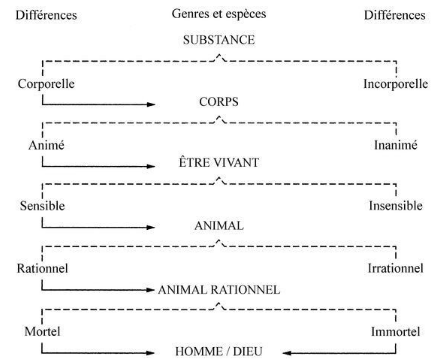
\includegraphics[width=12cm]{images/arbre_porprhyre_differences.png}
	\caption[Arbre porphyrien prenant en compte les différences]{Arbre porphyrien prenant en compte les différences [Source: \cite[chap.1]{eco_arbre_2010}]}
	\label{arbre_porphyre_differences}
\end{figure}

Cependant, si la prise en compte des différences permet de différencier l'homme du cheval, elles ne permettent pas de distinguer le cheval de l'âne par exemple. Un même genre doit donc être utilisé plusieurs fois dans l'arbre, ce qui le rend infini, et l'établissement d'un dictionnaire impossible à réaliser (voir \reference{arbre_porphyre_boucle}).\\

\begin{figure}[!h]
	\centering
	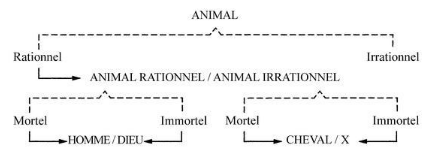
\includegraphics[width=12cm]{images/arbre_porphyre_boucle.png}
	\caption[Infinitude de l'arbre de Porphyre]{Infinitude de l'arbre de Porphyre [Source: \cite[chap.1]{eco_arbre_2010}]}
	\label{arbre_porphyre_boucle}
\end{figure}

Face à cette impossibilité de décrire le monde avec des divisions uniques dans un seul arbre, c'est à dire d'établir un dictionnaire universel, absolu et global, la seule solution paraît être la création d'un nombre d'arbres infini, composés de propriétés s'articulant selon le contexte et le domaine d'utilisation de l'arbre: d'un seul arbre insaisissable, une forêt réorganisable à l'envi et à l'infini est apparue, laissant le choix à l'utilisateur de l'arbre utilisé selon le sujet.

\subsection{\label{I-C-1-b}L'encyclopédisme (Antiquité - Moyen-Âge): la recherche d'un arbre global mimant le monde réel}
\titreEntete{L'encyclopédisme}

L'utopie de saisie totale du monde se retrouve dans l'encyclopédisme, dès l'\textit{Historia naturalis} de \nP{Pline}{l'Ancien}. Sur le même principe que l'arbre porphyrien, la hiérarchie de l'index de cette encyclopédie de 37 volumes part de l'original vers le dérivé, du naturel à l'artifice: \og Une encyclopédie, pour s’organiser, tente de suivre le modèle de l’arbre --- qui est toujours plus ou moins consciemment celui de la subdivision binaire d’un arbre porphyrien\fg{}\footnote{\cite[chap.1]{eco_arbre_2010}. Voir \reference{index_pline}}. Cependant, l'index d'une encyclopédie se distingue des termes d'un arbre porphyrien en ce qu'il est défini dans un autre développement --- un article d'encyclopédie ---, alors que les termes de l'arbre de Porphyre ne peuvent pas être définis par la suite.

\begin{figure}[!h]
	\centering
	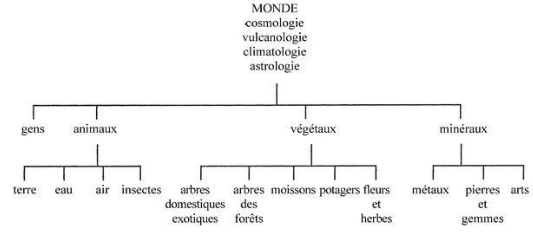
\includegraphics[width= 13cm]{images/index_pline.png}
	\caption{Extrait de l'arborescence de l'index de \nP{Pline}{l'Ancien}}
	\label{index_pline}
\end{figure}

Avec le passage au christianisme, l'encyclopédisme doit décrire les textes sacrés et non plus le monde. Ainsi, des éléments moralisateurs et allégoriques se retrouvent dans les index, devant les éléments matériels du monde\footnote{La tradition moralisatrice encyclopédique naît avec le \textit{Physiologos} d'un auteur grec et s'inspire de l'œuvre de \nP{Pline}{l'Ancien}, et se poursuit tout au long du Moyen-Âge avec les \textit{Étymologies} d'\nP{Isidore}{de Séville} notamment.}. À partir du \textsc{XIII}\textsuperscript{ème}siècle, les encyclopédies montrent l'ordre qui les dirige: cela conduit à \textit{L'arbre de science} de \nP{Raymond}{Lulle} qui créé seize arbres représentant l'Être, chacun représentant un savoir différent en se divisant en sept parties (racines, tronc, branches, rameaux, feuilles, fleurs, fruits)\footcite[chap.10]{eco_arbre_2010}. Contrairement à l'arbre de Porphyre qui est un arbre vide que l'on peut remplir selon le contexte, les arbres que propose \nP{Raymond}{Lulle} sont pleins et ont pour vocation de décrire et de classer le monde, la Grande Chaîne de l'Être.

\subsection{\label{I-C-1-c}Influences: une diversité de référentiels hiérarchiques}
\titreEntete{Influences: une diversité de référentiels hiérarchiques}

La pensée aristotélicienne puis le commentaire porphyrien ont produit une tradition de hiérarchisation du monde qui s'est poursuivie pendant plus d'un millénaire, sans cesse confrontée à l'impossibilité d'une description totale de ce monde. La multiplicité des arbres est, chez \nP{Umberto}{Eco} puis dans celle de \nP{Raymond}{Lulle}, la conclusion de leur réflexion. L'influence de cette tradition de description est sensible jusqu'à aujourd'hui, notamment dans le domaine de l'indexation et de la bibliothéconomie.\\

En effet, une diversité de référentiels est apparue, chacun étant dérivé d'un arbre. Des schémas de classification sont définissables à l'infini, emboîtant les genres, les espèces et les différences\footnote{\og Un simple artifice classificatoire consiste à emboîter des genres, des espèces et des différences sans en expliquer le \textit{definiendum}\fg{} in \cite[chap.1]{eco_arbre_2010}}. La taxonomie naît de ce modèle d'arbre: la taxonomie n'a pas pour but de dire comment repérer le concept décrit, elle permet seulement de classer en renvoyant, pour chaque nœud, vers un autre chapitre où l'on décrit ces propriétés. La taxonomie, bien qu'historiquement appliquée aux sciences de la terre, a été reprise par \nP{Melvil}{Dewey} dans sa classification décimale \index[referentiels]{dewey@Dewey} en 1876.\\

Définie comme un \og classement hiérarchique de termes préférentiels\fg{} par \nP{Louis}{Rosenfeld} et \nP{Peter}{Morville}\footcite{rosenfeld_information_2015}, la taxonomie ne veut pas définir, mais simplement permettre l'utilisation correcte et logique du terme par l'attribution de catégories et l'utilisation exclusive de relations hiérarchiques.\\

Les \textit{thesauri}\footnote{Ils sont décrits comme une \og liste organisée de termes contrôlées et normalisés (descripteurs et non-descripteurs) servant à l’indexation des documents et des questions dans un système documentaire\fg{} dans \cite{degez_thesauroglossaire_2001}. Peu formels, ils sont néanmoins le vocabulaire le plus utilisé pour l'indexation. L'un des \textit{thesauri} les plus utilisés est le \ac{gemet}(\cite{noauthor_general_nodate}). Le \index[referentiels]{gemet@GEMET} est disponible en plus de trente langues et diffusé par l'Agence européenne de l'Énergie. Voir \reference{I-C-2}.} utilisent plus de relations et de types de termes, de manière à indexer des contenus avec des mots-clés et à faciliter la recherche. Ce vocabulaire contrôlé hiérarchique reste proche du langage naturel en y intégrant les variantes, les synonymes, les descriptions, les traductions et les équivalences.\\

Pour avoir une plus grande formalisation du thésaurus, il faut utiliser une ontologie. Cette ontologie est la spécification formelle d'un espace de noms, d'un domaine particulier de la connaissance\footnote{L'une des ontologies les plus utilisées, notamment dans le web sémantique, est \ac{foaf}. \index[referentiels]{foaf@FOAF} permet la description précise des personnes. Voir \cite{noauthor_foaf_nodate}}. Elle identifie alors les objets à décrire, leurs relations au sein de ce domaine ainsi que leurs propriétés. L'ontologie n'est pas utilisée directement dans l'indexation ou la recherche, elle est d'abord utilisée pour instancier et raisonner, en s'éloignant du langage naturel avec l'utilisation d'identifiants techniques.\\

Les taxonomies, les \textit{thesauri} ainsi que les ontologies héritent tous du modèle de l'arbre, la description ou la classification par la hiérarchie étant la plus efficace pour ces besoins. Ces vocabulaires sont les plus complexes par les relations qui les composent. \nP{Louis}{Rosenfeld} et \nP{Peter}{Morville}\footnote{\cite{rosenfeld_information_2015}. Voir \reference{frise_voca}} considèrent l'anneau de synonymie comme le plus simple des vocabulaires, avec des relations d'équivalence, alors que les fichiers d'autorité et les taxonomies, fonctionnant sur la hiérarchie, sont plus complexes. Les \textit{thesauri} et les ontologies sont plus complexes encore puisqu'ils sont constitués de relations hiérarchiques et associatives.

\begin{figure}[!h]
	\centering
	
	\begin{pspicture}(0,2)(10,8)
		\psline[linewidth=1.5pt]{->}(0,5)(10,5)
		\uput[0](-2.5,5){\textsc{Simple}}
		\uput[0](10.5,5){\textsc{Complexe}}
		\uput[0](3,3){\textbf{\textsc{Type de relations}}}
		\uput[0](2.5,7){\textbf{\textsc{Type de vocabulaire}}}
		\uput[0](0,4){Équivalence}
		\uput[0](3.8,4){Hiérarchique}
		\uput[0](7.6,4){Associative}
		\uput[0](-1,6.3){Anneau de synonymie}
		\uput[0](2.5,5.5){Fichiers d'autorité}
		\uput[0](5,6.1){Taxonomies}
		\uput[0](7,5.5){Thésaurus}
		\uput[0](9,6.3){Ontologies}
	\end{pspicture}
	
	\caption[Classification des vocabulaires selon leur complexité]{Classification des vocabulaires selon leur complexité [d'après \cite{rosenfeld_information_2015}]}
	\label{frise_voca}
\end{figure}

\section{\label{I-C-2}Le \textit{thésaurus}, vocabulaire contrôlé hiérarchique le plus fréquent}
\titreEntete{Le thésaurus}

Né dans les années 1950 aux États-Unis, le \index[ref]{typologie@Typologie!thesaurus@Thésaurus}thésaurus n'a été adopté massivement qu'avec l'apparition de l'informatique. C'est un langage combinatoire, une liste organisée de termes normalisés et contrôlés, qui permet de faire le lien entre le langage naturel de l'homme et le nécessaire besoin d'avoir un langage contrôlé pour les ressources. La sélection d'un terme lors de l'indexation permet de sélectionner un concept lui-même décrit par plusieurs termes (synonymes, équivalents, traductions). Ainsi, les institutions patrimoniales se sont emparées de cet outil, adaptable au domaine de chacune: l'\ac{ina} possède un thésaurus orienté vers l'audiovisuel, la Cinémathèque française un \href{http://www.cineressources.net/thesaurus/}{thésaurus orienté vers le cinéma}.

\subsection{\label{I-C-2-a}Types de structure}
\titreEntete{Types de structure}

Le type de \index[ref]{typologie@Typologie!thesaurus@Thésaurus}thésaurus le plus utilisé est celui constitué d'une hiérarchie simple\footnote{La typologie des \textit{thesauri} décrite par la suite est présente chez \cite{rosenfeld_information_2015}.}. L'\ac{ina} possède un thésaurus de noms communs formé sur cette hiérarchie simple à unique ascendance\footnote{Voir \reference{annexe_thesaurus}}, c'est à dire qu'un terme est nécessairement descendant d'une seule classe, il ne peut pas hériter de deux caractéristiques différentes, ce qui le rapproche de la \index[ref]{typologie@Typologie!taxonomie@Taxonomie}taxinomie\footnote{Voir \reference{modele_taxo} et \reference{modele_thes_simple}.}.

\begin{figure}[!h]
	\begin{minipage}[c]{.46\linewidth}
			\centering
			\begin{pspicture}(0,2.5)(6.5,7)
				\psframe[fillstyle=solid,fillcolor=lightgray](0,6)(1.5,6.5)
				\psframe[fillstyle=solid,fillcolor=lightgray](1.5,5)(3,5.5)
				\psframe[fillstyle=solid,fillcolor=lightgray](3,4)(4.5,4.5)
				\psframe[fillstyle=solid,fillcolor=lightgray](4.5,3)(6,3.5)
				\psline{->}(0.75,6)(0.75,5.2)(1.5,5.2)
				\psline{->}(2.25,5)(2.25,4.2)(3,4.2)
				\psline{->}(3.75,4)(3.75,3.2)(4.5,3.2)
			\end{pspicture}
			\caption{Le modèle taxonomique}
			\label{modele_taxo}
	\end{minipage}
	\begin{minipage}[c]{.46\linewidth}
			\centering
			\begin{pspicture}(0,1.5)(7,7)
			\psframe[fillstyle=solid,fillcolor=lightgray](3,6.5)(4.5,7)
			\psline{->}(3.75,6.5)(3.75,5.5)
			\psframe[fillstyle=solid,fillcolor=lightgray](3,5)(4.5,5.5)
			\psline(3.75,5)(3.75,4.5)
			\psframe[fillstyle=solid,fillcolor=lightgray](1.5,3.5)(3,4)
			\psline{->}(3.75,4.5)(2.25,4.5)(2.25,4)
			\psframe[fillstyle=solid,fillcolor=lightgray](4.5,3.5)(6,4)
			\psline{->}(3.75,4.5)(5.25,4.5)(5.25,4)
			\psframe[fillstyle=solid,fillcolor=lightgray](0.75,2)(2.25,2.5)
			\psline{->}(2.25,3.5)(2.25,3)(1.5,3)(1.5,2.5)
			\psline(5.25,3.5)(5.25, 3)
			\psframe[fillstyle=solid,fillcolor=lightgray](3.5,2)(5,2.5)
			\psline{->}(5.25, 3)(4.25,3)(4.25,2.5)
			\psframe[fillstyle=solid,fillcolor=lightgray](5.5,2)(7,2.5)
			\psline{->}(5.25, 3)(6.25,3)(6.25,2.5)
			\end{pspicture}
			\caption{Le modèle du thésaurus simple}
			\label{modele_thes_simple}
	\end{minipage}
	\medskip
	\\
	\caption*{Comparaison entre le modèle taxonomique et celui du thésaurus à hiérarchie simple [d'après \cite{rosenfeld_information_2015}]}
\end{figure} 

De manière à exprimer la descendance depuis plusieurs caractéristiques, un thésaurus polyhiérarchique existe. Il permet de définir et d'accepter plus de termes contrôlés que le thésaurus simple. En effet, par la combinaison des termes ascendants, un même terme peut avoir deux ascendances différentes. \nP{Peter}{Morville} et \nP{Louis}{Rosenfeld} prennent un exemple médical pour illustrer ce type particulier de thésaurus.

\begin{figure}[!h]
	\begin{minipage}[c]{.46\linewidth}
			\centering
			\begin{pspicture}(0,1.75)(7,8.75)
			\psframe[fillstyle=solid,fillcolor=lightgray](1.5,8)(3,8.5)
			\psline{->}(3.75,7.5)(3.75,7)
			\psline(3.75,7.5)(2.25,7.5)(2.25,8)
			\psframe[fillstyle=solid,fillcolor=lightgray](4.5,8)(6,8.5)
			\psline(3.75,7.5)(5.25,7.5)(5.25,8)
			\psframe[fillstyle=solid,fillcolor=lightgray](3,6.5)(4.5,7)
			\psline{->}(3.75,6.5)(3.75,5.5)
			\psframe[fillstyle=solid,fillcolor=lightgray](3,5)(4.5,5.5)
			\psline(3.75,5)(3.75,4.5)
			\psframe[fillstyle=solid,fillcolor=lightgray](1.5,3.5)(3,4)
			\psline{->}(3.75,4.5)(2.25,4.5)(2.25,4)
			\psframe[fillstyle=solid,fillcolor=lightgray](4.5,3.5)(6,4)
			\psline{->}(3.75,4.5)(5.25,4.5)(5.25,4)
			\psframe[fillstyle=solid,fillcolor=lightgray](0.75,2)(2.25,2.5)
			\psline{->}(2.25,3.5)(2.25,3)(1.5,3)(1.5,2.5)
			\psline(5.25,3.5)(5.25, 3)
			\psframe[fillstyle=solid,fillcolor=lightgray](3.5,2)(5,2.5)
			\psline{->}(5.25, 3)(4.25,3)(4.25,2.5)
			\psframe[fillstyle=solid,fillcolor=lightgray](5.5,2)(7,2.5)
			\psline{->}(5.25, 3)(6.25,3)(6.25,2.5)
			\end{pspicture}
			\caption{Le modèle polyhiérarchique}
			\label{modele_polyh}
		\end{minipage}
	\begin{minipage}[c]{.46\linewidth}
	\centering
	\begin{pspicture}(0,1.75)(5,6)
		\psframe[fillstyle=solid,fillcolor=lightgray](1.75,5)(3.25,5.5)
		\psline(2.5,5)(2.5,4.5)
		\uput[0](1.75,5.25){Décès}
		\psframe[fillstyle=solid,fillcolor=lightgray](0.75,3.5)(2.25,4)
		\psline{->}(2.5,4.5)(3.5,4.5)(3.5,4)
		\uput[0](0.75,3.75){Virus}
		\psframe[fillstyle=solid,fillcolor=lightgray](2.75,3.5)(4.25,4)
		\psline{->}(2.5,4.5)(1.5,4.5)(1.5,4)
		\uput[0](2.6,3.75){\scriptsize{Respiration}}
		\psframe[fillstyle=solid,fillcolor=lightgray](1.75,2)(3.25,2.5)
		\uput[0](1.6,2.25){\scriptsize{Pneumonie}}
		\psline(1.5,3.5)(1.5,3)(2.5,3)
		\psline(3.5,3.5)(3.5,3)(2.5,3)
		\psline{->}(2.5,3)(2.5,2.5)
	\end{pspicture}
	\caption{Application du modèle polyhiérarchique}
	\label{application_polyh}
\end{minipage}
\medskip
\\
\caption*{Le modèle du thésaurus polyhiérarchique [d'après \cite{rosenfeld_information_2015}]}
\end{figure}

Enfin, comme nous l'avons évoqué précédemment\footnote{Voir \reference{I-C-1}.}, le seul arbre possible est un arbre multiple, adapté à son contexte. Ainsi, des \textit{thesauri} à facettes existent, reflétant les multiples dimensions thématiques que peuvent contenir les documents ou les éléments: un terme se retrouve alors dans plusieurs arbres, multipliant les points d'accès. Plusieurs \index[ref]{typologie@Typologie!thesaurus@Thésaurus}\textit{thesauri} simples sont par conséquent créés, permettant la description de l'ensemble de ces dimensions.

\subsection{\label{I-C-2-b}Relations entre les termes}
\titreEntete{Relations entre les termes}

La force du \index[ref]{typologie@Typologie!thesaurus@Thésaurus}thésaurus ne réside pas seulement dans l'enchaînement d'ascendances et de descendances. Les relations établies entre les termes sont essentielles pour permettre le lien entre le langage humain naturel et le besoin de contrôle imposé par l'indexation et la recherche: un thésaurus est \og un vocabulaire contrôlé dans lequel les relations d'équivalence, de hiérarchie et d'association sont correctement identifiées de manière à permettre une meilleure récupération\fg{}\footcite{rosenfeld_information_2015}.\\

Les relations créées précisent le sens de chaque vedette par comparaison aux vedettes de sens voisin, elles permettent de naviguer entre ces vedettes pour affiner sa recherche, l'élargir ou bien la réorienter. La hiérarchisation et l'établissement de liens permettent de passer à une navigation sémantique, alors que les simples vocabulaires contrôlés évoqués au \reference{I-A} ne permettaient qu'une navigation par mots.\\

La première relation est la relation d'équivalence.
\begin{wrapfigure}{L}{4cm}
	\centering
	\begin{pspicture}(0,0)(2.6,2.6)
	\pscircle(1.3,1.3){1.3}
	\uput[0](0.5,1.3){A~=~B}
\end{pspicture}
	\caption{Relation d'équivalence}
	\label{relation_equivalence}	
\end{wrapfigure} Elle connecte le terme préférentiel --- le terme principal de la vedette --- à ses variantes: les synonymes, les acronymes, les abréviations, les variantes lexicales ou les différences de graphie sont ainsi incorporés au thésaurus comme variantes. Cette relation\footnote{Voir \reference{relation_equivalence}} est une relation horizontale, d'égalité, comme dans l'anneau de synonymie. Dans l'\reference{annexe_thesaurus}, le terme \og Cadreur\fg{}, qui est le terme préférentiel, a deux variantes --- ou termes \og Employés pour\fg{}, \og Cameraman\fg{} et \og Opérateur de prise de vue\fg{}.\\

Le second type de relation est la relation associative. \begin{wrapfigure}{R}{5cm}
	\centering
	\begin{pspicture}(0,0)(4.6,2.6)
	\pscircle(1.3,1.3){1.3}
	\uput[0](0.6,1.3){A}
	
	\pscircle(3.2,1.3){1.3}
	\uput[0](3,1.3){B}
\end{pspicture}
	\caption{Relation d'association}
	\label{relation_association}	
\end{wrapfigure} Comme la relation d'équivalence, elle est horizontale. Elle permet d'exprimer la proximité sémantique entre deux termes: dans \index[ref]{lod@Linked Open Data (LOD)!rameau@RAMEAU}\index[ref]{autorites@Autorités!rameau@RAMEAU}\ac{rameau}, la vedette \href{https://data.bnf.fr/fr/11933646/television/}{\og Télévision\fg{}} possède quarante relations d'association avec d'autres vedettes, comme \href{https://data.bnf.fr/fr/12648926/industrie_de_la_television/}{\og Industrie de la télévision\fg{}}. L'association\footnote{Voir \reference{relation_association}.} n'est pas une relation de stricte égalité, elle indique le partage sémantique d'une partie de leur définition. Cette relation permet l'élargissement d'une recherche depuis une vedette.\\

Le dernier type de relation est hiérarchique. Il est le plus utilisé car il permet l'expression de nombreuses relations du langage naturel: \begin{wrapfigure}{L}{5cm}
	\centering
	\begin{pspicture}(0,0)(2.6,2.6)
	\pscircle(1.3,1.3){1.3}
	\uput[0](0.6,1.6){A}
	
	\pscircle(1.5,1){0.5}
	\uput[0](1.1,1){B}
\end{pspicture}
	\caption{Relation de hiérarchie}
	\label{relation_hierar}	
\end{wrapfigure}
\begin{itemize}
	\item la relation génétique --- la plus fréquente --- peut ainsi être exprimée. Le sens du terme générique est inclus dans celui du terme spécifique: la vedette \index[ref]{lod@Linked Open Data (LOD)!rameau@RAMEAU}\index[ref]{autorites@Autorités!rameau@RAMEAU}\ac{rameau} \href{https://data.bnf.fr/fr/11960499/radiodiffusion/}{\og Radiodiffusion\fg{}} est l'un des termes génériques de  \href{https://data.bnf.fr/fr/11933646/television/}{\og Télévision\fg{}} qui est elle-même terme générique de \href{https://data.bnf.fr/fr/11936935/chaines_de_television/}{\og Chaînes de télévision\fg{}} notamment. Chacune de ces vedettes est décrite par son ascendance et sa descendance.
	\item la relation d'appartenance --- ou de regroupement --- est possible;
	\item la relation partitive
\end{itemize}
La définition de cette relation hiérarchique\footnote{Voir \reference{relation_hierar}.} permet l'expression de caractéristiques et de relations infinies du langage naturel. La recherche d'une vedette peut alors être affinée --- quand l'utilisateur passe d'une vedette générique à une vedette spécifique --- ou bien élargie --- quand il passe d'une vedette spécifique à une vedette générique.\\

Alors, chaque terme devient le centre de son propre réseau et construit un nouvel arbre, entièrement né de son contexte.


\subsection{\label{I-C-2-c}Utiliser la précoordination pour les relations complexes}
\titreEntete{Utiliser la précoordination pour les relations complexes}

L'inconvénient du \index[ref]{typologie@Typologie!thesaurus@Thésaurus}thésaurus comme évoqué précédemment est l'impossibilité pour l'utilisateur de feuilleter \index[ref]{typologie@Typologie!index@Index}l'index: \og Télévision\fg{} et \og Chaînes de télévision\fg{}, bien qu'étant proches, ne seraient pas au même endroit dans l'index. Pour faciliter la navigation de l'utilisateur, les mots-clés sont coordonnés avant l'utilisation par l'utilisateur pour former une vedette-matière construite (comme dans le cas de \index[ref]{lod@Linked Open Data (LOD)!rameau@RAMEAU}\index[ref]{autorites@Autorités!rameau@RAMEAU}\ac{rameau}): une vedette principale constitue la tête de la vedette, puis des subdivisions la complètent\footnote{Dans \og \href{https://data.bnf.fr/fr/11977461/plantes-hotes/}{Plantes -- Parasites -- Plantes-hôtes}\fg{}, \og Plantes\fg{} est la tête de vedette, complétée par deux subdivisions.}. Une vision globale est ainsi offerte et permet une précision du sujet des facettes ainsi qu'une limitation du bruit: \href{https://data.bnf.fr/fr/11977461/plantes-hotes/}{Plantes -- Parasites -- Plantes-hôtes}\fg{} est ainsi séparée de \href{https://data.bnf.fr/fr/12397201/plantes_parasites/}{\og Plantes parasites\fg{}}.\\

\bigskip
\bigskip
Les différentes structures de \index[ref]{typologie@Typologie!thesaurus@Thésaurus}\textit{thesauri} et leurs multiples relations permettent un modèle de classification, de combinaison et de description efficace des termes, à la fois proche du langage naturel mais en s'en éloignant par le formalisme et le contrôle des termes. Chaque vedette est le centre de son propre référentiel, dirigeant vers des variantes, des vedettes proches ou en relation.

\begin{figure}[!h]
	\centering
	
	\begin{pspicture}(0,0)(15,7.6)
		\psline{->}(7.5,3)(7.5,3.5)
		\psframe[fillstyle=solid,fillcolor=lightgray](0,0)(3,1)
		\uput[0](0.8,0.8){Terme}
		\uput[0](0.9,0.3){relatif}
		\psline{->}(1.5,2)(1.5,1)
		\uput[0](0.3,2.8){Relation d'}
		\uput[0](0.3,2.3){association}
		\psline(2.5,3)(7.5,3)
		\psframe[fillstyle=solid,fillcolor=lightgray](6,0)(9,1)
		\uput[0](6.8,0.8){Terme}
		\uput[0](6.5,0.3){spécifique}
		\psline{->}(7.5,1.5)(7.5,1)
		\uput[0](6.6,2.3){Relation}
		\uput[0](6.3,1.8){hiérarchique}
		\psline(7.5,3)(7.5,2.5)
		\psframe[fillstyle=solid,fillcolor=lightgray](12,0)(15,1)
		\uput[0](12.8,0.8){Terme}
		\uput[0](12.9,0.3){relatif}
		\psline{->}(13.5,2)(13.5,1)
		\uput[0](12.5,2.8){Relation d'}
		\uput[0](12.3,2.3){association}
		\psline(12,3)(7.5,3)
		
		\psframe[fillstyle=solid,fillcolor=lightgray](0,3.5)(3,4.5)
		\uput[0](0.5,4){Variante}
		\psline{->}(3.5,4)(3,4)
		\uput[0](3.5,4.2){Relation d'}
		\uput[0](3.5,3.8){équivalence}
		\psline{->}(5.5,4)(6,4)
		\psframe[fillstyle=solid,fillcolor=lightgray](6,3.5)(9,4.5)
		\uput[0](6.8,4.2){Terme}
		\uput[0](6.5,3.8){préférentiel}
		\psframe[fillstyle=solid,fillcolor=lightgray](12,3.5)(15,4.5)
		\uput[0](12.5,4){Variante}
		\psline{->}(9.5,4)(9,4)
		\uput[0](9.5,4.2){Relation d'}
		\uput[0](9.5,3.8){équivalence}
		\psline{->}(11.5,4)(12,4)
		
		\psframe[fillstyle=solid,fillcolor=lightgray](6,6.5)(9,7.5)
		\uput[0](6.8,7.2){Terme}
		\uput[0](6.5,6.7){générique}
		\psline{->}(7.5,5)(7.5,4.5)
		\psline{->}(7.5,6)(7.5,6.5)
		\uput[0](6.6,5.6){Relation}
		\uput[0](6.3,5.2){hiérarchique}
	\end{pspicture}
	\caption[Modélisation d'une vedette de thésaurus]{Modélisation d'une vedette de thésaurus [d'après \cite{rosenfeld_information_2015}]}
	\label{modelisation_thes}
\end{figure}

\section[Passer du texte libre à un vocabulaire contrôlé: aligner des notes qualités et un thésaurus de noms communs]{\label{I-C-3}Passer du texte libre à un vocabulaire contrôlé}
\titreEntete{Passer du texte libre à un vocabulaire contrôlé}

Dans la description de documents audiovisuels --- comme dans celle d'autres documents patrimoniaux ---, désigner des personnes est indispensable. Pour enrichir le seul état civil de la personne, plusieurs moyens peuvent être utilisés:
\begin{itemize}
	\item rédiger un texte libre décrivant les caractéristiques de la personne, ses fonctions, ses dates de naissance et de mort, \dots. Cette solution pose la problématique de la structuration des données: un texte libre n'est pas lisible par une machine; son accès est par conséquent restreint.
	\item utiliser un \index[ref]{typologie@Typologie!vocabulaires controles@Vocabulaires contrôlés}vocabulaire contrôlé et sélectionner les termes correspondant à la personne. Cependant, en fonction du niveau de précision souhaité, ce vocabulaire doit être plus ou moins précis, rendant, dans le cas d'une grande précision, la description longue et fastidieuse.
	\item définir des champs essentiels à la description de cette personne, et rédiger un texte libre pour les informations supplémentaires. De même que dans le premier cas, le texte libre appauvrit l'effort de structuration de la description.
\end{itemize}
Face à ces difficultés, les documentalistes de la \ac{ddcol} à l'\ac{ina} ont créé des vedettes de personnes selon une succession de champs (sexe, date de naissance, date de mort, \dots) et de notes, dont une note qualité qui est régie par un guide de rédaction. Cette note qualité a pour but de décrire en quelques mots les fonctions de la personne et le lieu d'exercice. Cette note n'étant pas un point d'accès, elle peut être structurée et rédigée en texte libre.\\

Dans le cadre de la migration des données de la \ac{ddcol} dans le \ldd, un alignement de ces notes qualités est nécessaire avec le \index[ref]{typologie@Typologie!thesaurus@Thésaurus}thésaurus des noms communs qui existe parallèlement, notamment pour enrichir le thésaurus des fonctions des notes qualités qui n'y existent pas.

\subsection{\label{I-C-3-a}Contrôler du texte libre}
\titreEntete{Contrôler du texte libre}

La note qualité est rédigée selon des règles définies au préalable par les documentalistes. Cependant, la rédaction en texte libre conduit à l'apparition d'erreurs humaines, comme les erreurs de graphie, de grammaire ou de ponctuation. En effet, une note qualité peut avoir deux formes:
\begin{itemize}
	\item Fonction1, fonction2, \dots~. Pays
	\item Homonymes: 1 - Fonction1, fonction2, \dots~. Pays1, Pays2, \dots; 2 - Fonction1, fonction2, \dots~. Pays 
\end{itemize}
Ainsi, l'oubli d'une ponctuation, ou son inversion, conduit à rendre la note qualité non conforme aux règles et, par conséquent, à rendre son traitement plus difficile voire impossible. De plus, les différences de graphie liées au masculin et au féminin, ainsi qu'au singulier et au pluriel, rendent ces notes qualités très différentes.\\

De manière à pouvoir les aligner avec le \index[ref]{typologie@Typologie!thesaurus@Thésaurus}thésaurus des noms communs, un premier traitement est nécessaire, pour extraire et normaliser les fonctions. Le logiciel ETL (\textit{Extract Transform Loaad})\footnote{Un ETL permet de migrer des données depuis une source vers une cible, en leur appliquant des traitements avant de les charger dans la cible.} \href{https://www.talend.com/fr/products/big-data/}{Talend Big Data Platform} permet ce premier traitement.\\

La première étape consiste à scinder chaque note selon les fonctions et les pays: le point sépare ces deux éléments et permet cette scission. Ainsi, la fonction extraite de \og Historien, musicologue. France\fg{} est \og Historien, musicologue\fg{} alors que la note qualité \og Journaliste, France\fg{} ne peut pas être scindée correctement. Une seconde scission intervient par la suite de manière à récupérer chaque fonction une à une, passant de \og Historien, musicologue\fg{} à \og Historien\fg{} et \og musicologue\fg{}.\\

Quand les fonctions sont récupérées, le contrôle des termes peut avoir lieu selon plusieurs choix à effectuer en amont:
\begin{itemize}
	\item le choix du genre doit être effectué pour éviter les termes équivalents dans le sens mais différents en graphie
	\item le choix du nombre
	\item la gestion de la ponctuation propre aux fonctions comme les traits d'union
	\item la gestion de l'accentuation
\end{itemize}
Pour normaliser le plus possible, le choix du masculin singulier, de la suppression de toute la ponctuation et de l'accentuation ont été effectué. Pour les choix du genre, le nombre des exceptions comme \og musée\fg{}, portant une terminaison du féminin, étant plus faible que le nombre de tous les féminins, le choix du masculin s'est imposé pour normaliser le maximum de fonctions. La \autoref{exemple_realisateur_NQ} montre une dernière normalisation à effectuer: la suppression des \textit{stopwords}, effectuée en \autoref{exemple_realisateur_NQ2}.
\begin{table}[!h]
	\centering
	\csvautotabular[separator=semicolon]{images/dessinateur_fonctions.csv}
	\caption{Données d'exemple de notes qualités avec la fonction de Réalisateur}
	\label{exemple_realisateur_NQ}
\end{table}
\begin{table}[!h]
	\centering
	\csvautotabular[separator=semicolon]{images/dessinateur_fonctions2.csv}
	\caption{Données d'exemple de notes qualités avec la fonction de Réalisateur, après normalisation des fonctions}
	\label{exemple_realisateur_NQ2}
\end{table}
\bigskip

Après la normalisation, les fonctions sont suffisamment contrôlées et proches des règles d'un \index[ref]{typologie@Typologie!thesaurus@Thésaurus}thésaurus pour être alignées. Cependant, nous pouvons observer que les erreurs humaines de graphie, comme l'oubli d'un \og s\fg{} dans \og dessinateur\fg{}, restent et ne permettront pas, par conséquent, d'être alignées. Le traitement correct de l'ensemble des notes en texte libre reste impossible suite aux erreurs introduites par l'homme.\\

Enfin, les notes qualités de l'\ac{ina} comprennent également des qualités ne décrivant pas directement la personne, mais définissant cette personne par un lien avec un fait. C'est le cas des faits divers, des attentats, des affaires judiciaires dans lesquels une personne peut être impliquée comme victime, accusée, témoin, \dots; c'est le cas également des indications de filiation et de généalogie avec lesquelles une personne est seulement désignée, sans apporter de précisions sur ses véritables fonctions\footnote{Voir \reference{exemple_NQ_sans_fonctions}.}. Ces parties de notes qualités --- ou bien la totalité de ces notes --- ne décrivant pas la fonction de la personne et n'allant pas trouver d'équivalent dans le \index[ref]{typologie@Typologie!thesaurus@Thésaurus}thésaurus, elles sont écartées du traitement.
\begin{table}[!h]
	\centering
	\csvautotabular[separator=semicolon]{images/affaires_attentat.csv}
	\caption{Données d'exemple de notes qualités sans fonctions}
	\label{exemple_NQ_sans_fonctions}
\end{table}

\subsection{\label{I-C-3-b}Aligner les extractions en langage naturel avec un thésaurus de noms communs}
\titreEntete{Aligner avec un thésaurus de noms communs}

Avec le premier traitement de normalisation des fonctions, les notes qualités sont sorties du langage naturel de manière à pouvoir être contrôlées dans un vocabulaire plus strict. L'alignement avec le \index[ref]{typologie@Typologie!thesaurus@Thésaurus}thésaurus de noms communs peut alors être réalisé\footnote{De manière à avoir la même normalisation de chaque côté de l'alignement, le thésaurus a subi le même traitement que les notes qualité, avec l'application des mêmes règles.}. Ce thésaurus est classé dans un ordre hiérarchique, mais l'accès par des termes ascendants est difficile pour l'alignement: les termes génériques sont souvent des noms qui ne sont pas des fonctions, ce qui rend leur alignement impossible. Ainsi, le terme \og Dessinateur\fg{} a pour ascendance \og \$art et culture/arts plastiques/dessin\fg{}: \og Dessin\fg{} ou \og Arts plastiques\fg{} ne sont pas des fonctions. L'ensemble des alignements est par conséquent réalisé avec les termes préférentiels les plus bas dans l'arborescence. Le thésaurus contenant également des synonymes\footnote{Voir les termes \textit{Employés pour} dans l'\reference{annexe_thesaurus} (\reference{thesaurus_cadreur}).}, ces derniers sont utilisés dans l'alignement de manière à réduire encore l'impact du langage naturel des notes qualités sur la qualité de l'alignement.\\

Cette phase d'alignement est également réalisée avec Talend grâce à une succession de jointures\footnote{Ici, les jointures sont des \textit{inner join} pour aligner sur la similarité entre les deux côtés --- fonctions issues de la note qualité, et termes du thésaurus --- , ou bien des comparaison effectuées à partir du début de la fonction issue des notes qualités --- \og Illustrateur de presse\fg{} pourra ainsi correspondre au terme \og Illustrateur\fg{} du thésaurus.}. Les fonctions strictement égales au terme préférentiel du thésaurus sont ainsi alignées, ainsi que celles qui commencent par un terme du thésaurus. Cette étape de l'alignement montre les difficultés posées par l'utilisation du texte libre dans la description ainsi que la gestion impossible des coquilles, bien que parfois très proche du terme exact\footnote{Voir l'exemple de l'alignement du terme \og Journaliste\fg{} \reference{annexe_alignement_journaliste}.}.\\

Face à ces difficultés et au nombre peu élevé des alignements qui résultent de cette étape, l'utilisation des synonymes peut apporter des résultats supplémentaires: l'entrée \og Cuisinier\fg{} du \index[ref]{typologie@Typologie!thesaurus@Thésaurus}thésaurus de noms communs comprend un synonyme, \og Chef de cuisine\fg{}. Cependant, le nombre des synonymes est réduit, et des alignements sont ici aussi non réalisés\footnote{Voir \reference{alignement_cuisinier}}.
\begin{table}[!h]
	\centering
	\csvautotabular[separator=semicolon]{images/alignement_cuisinier.csv}
	\caption{Utilisation des synonymes pour l'alignement du terme \og Cuisinier\fg{}}
	\label{alignement_cuisinier}
\end{table}

Enfin, le cas de \og Chef cuisinier\fg{} montre la nécessité d'utiliser le second terme de l'expression de la fonction\footnote{Voir \reference{alignement_cuisinier_polysemie}}: cette dernière étape de l'alignement permet l'alignement des fonctions commençant par des termes polysémiques comme \og Chef\fg{}, \og Directeur\fg{}, \og Maître\fg{},\dots
\begin{table}[!h]
	\centering
	\csvautotabular[separator=semicolon]{images/alignement_cuisinier_polysemie.csv}
	\caption{Gestion de la polysémie dans l'alignement du terme \og Cuisinier\fg{}}
	\label{alignement_cuisinier_polysemie}
\end{table}

\subsection{\label{I-C-3-c}Classer selon le thésaurus}
\titreEntete{Classer selon le thésaurus}

L'utilisation des relations d'association a permis d'aligner les fonctions avec les termes du \index[ref]{typologie@Typologie!thesaurus@Thésaurus}thésaurus. Les relations de hiérarchie avec les termes génériques permettent de classer ces fonctions. Ainsi, elles sont utilisées pour définir huit catégories de rattachement dans les fonctions extraites des notes qualité, de manière à les classer selon le thésaurus. Dans le thésaurus des noms communs, huit termes permettent de rattacher l'ensemble des termes spécifiques, souvent avec des niveaux intermédiaires de hiérarchie\footnote{Ces huit catégories sont: \og Art et culture\fg{}, \og communication diffusion traitement information\fg{}, \og sciences\fg{}, \og sciences humaines\fg{}, \og sport\fg{}, \og vie économique\fg{}, \og vie quotidienne habitat alimentation et loisirs\fg et \og vie sociale\fg{}.}. Ces termes de catégorisation sont des facettes: ils ne sont pas attribuables directement à un concept à indexer, ils permettent le seul classement.\\

Cette opération de classement des fonctions des notes qualités selon l'arborescence du thésaurus permet, au-delà de l'ajout sémantique sur les termes alignés, de repérer les termes qui n'ont pas été alignés et d'en comprendre les raisons:
\begin{itemize}
	\item Des noms communs ne correspondant pas à des fonctions sont présents dans les notes qualité. Ainsi, des termes comme \og cirque pinder\fg{} ou \og clip
	\fg{} ne trouveront pas d'équivalence dans le thésaurus.
	\item Des noms trop spécifiques ne sont également pas présents: \og chemisier\fg{} est une fonction spécifique que les documentalistes pourront créer si nécessaire grâce à ce repérage dans les notes qualité.
	\item Des erreurs introduites par accident par l'homme empêchent certains alignements: c'est le cas par exemple de \og chercher\fg{} qui a un équivalent \og chercheur\fg{} dans le thésaurus. Il est difficile de repérer et de corriger ces erreurs automatiquement.
	\item La présence d'une documentation d'aide au catalogage et à l'indexation permet d'introduire de nouvelles règles dans la classification automatique: ainsi, \og designer interieur\fg{} peut être classifié dans la facette \og Art et culture\fg{} car la documentation l'indique; cependant, le terme \og designer\fg{} étant absent du \index[ref]{typologie@Typologie!thesaurus@Thésaurus}thésaurus, il ne peut pas être aligné.
\end{itemize}



%conclu
\bigskip
\bigskip
\bigskip
Aligner du texte libre avec un thésaurus nécessite plusieurs étapes et la prise en compte des différences de langage --- l'un étant un contrôle minimal du langage humain naturel, l'autre un vocabulaire contrôlé natif --- :
\begin{itemize}
	\item normaliser chaque côté de l'alignement selon les mêmes règles
	\item aligner selon l'exactitude avec le terme préférentiel
	\item aligner selon l'exactitude avec une variante du terme préférentiel
	\item aligner selon l'exactitude du commencement de la fonction avec le terme préférentiel
	\item aligner selon l'exactitude du commencement de la fonction avec une variante du terme préférentiel
	\item aligner selon l'exactitude du deuxième terme non polysémique de la fonction avec le terme préférentiel
\end{itemize}
	
	\part{\label{relier}RELIER. Vers le partage de référentiels communs (début des années 2000 – milieu des années 2010)}
	
	\chapter{\label{II-A}Le web de données: une exposition commune des référentiels}
	\titreEntete{Le web de données: une exposition commune des référentiels}
	\chapter{\label{II-B}Partager des structurations similaires de jeux de données par les classes et les propriétés : les ontologies, grammaires communes mais spécifiques}
	\titreEntete{Les ontologies, grammaires communes mais spécifiques}
	\chapter{\label{II-C}Relier ses données à Wikidata}
	\titreEntete{Relier ses données à Wikidata}
	
	\part{\label{centraliser}CENTRALISER. Le référentiel, clé de voûte et pivot (depuis le milieu des années 2010)}	
	
	\chapter{\label{III-A}Les labyrinthes comme réseaux de données et de liens}
	\titreEntete{Les labyrinthes comme réseaux de données et de liens}
	\chapter{\label{III-B}Le Lac de données de l’INA : le référentiel au centre du modèle}
	\titreEntete{Le référentiel au centre du modèle}
	\chapter{\label{III-C}Centraliser les référentiels de l’INA dans le Lac de données: l'exemple de l'alignement de deux référentiels de personnes physiques}
	\titreEntete{Aligner deux référentiels de personnes physiques}

	\chaptertoc{Conclusion}
\titreEntete{Conclusion}

%historique de struct ref: arbre au laby et modele reseau

%changement des usages et des besoins...

%... qui produit changement place ref
	
	\appendix
	\part*{Annexes}	
	\addcontentsline{toc}{part}{Annexes}
	\setcounter{chapter}{0}

\chapter{\label{annexe_index_schoepflin}Les index de la Renaissance, termes contrôlés et classification alphabétique (les index de l'\textit{Alsatia Illustrata} de \nP{Jean-Daniel}{Schoepflin})}
\titreEntete{Annexe \thechapter}

\begin{figure}[!h]
	\centering
	\begin{minipage}[c]{.46\linewidth}
		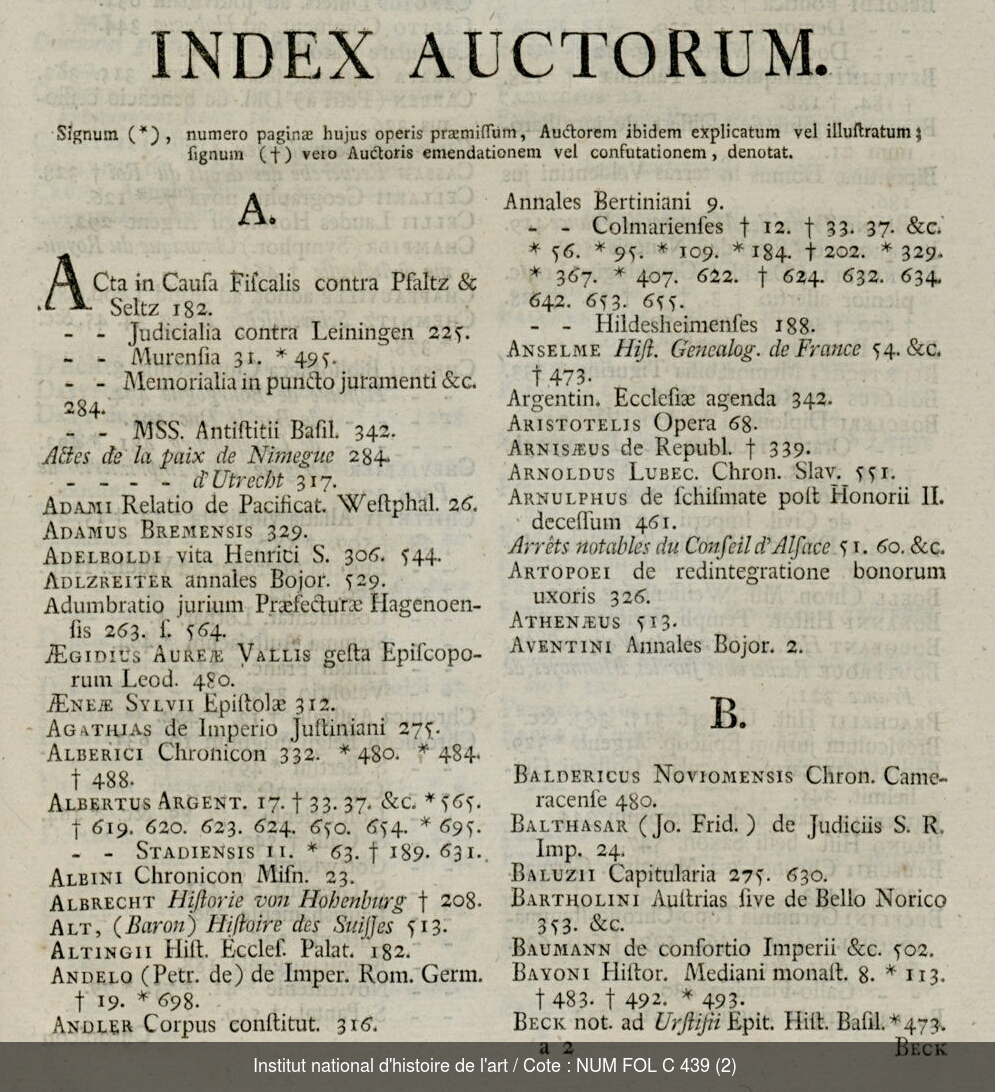
\includegraphics[width=6cm]{images/index_auctorum_alsatia.jpg}
		\caption{Index auctorum}
	\end{minipage} \hfill
	\begin{minipage}[c]{.46\linewidth}
		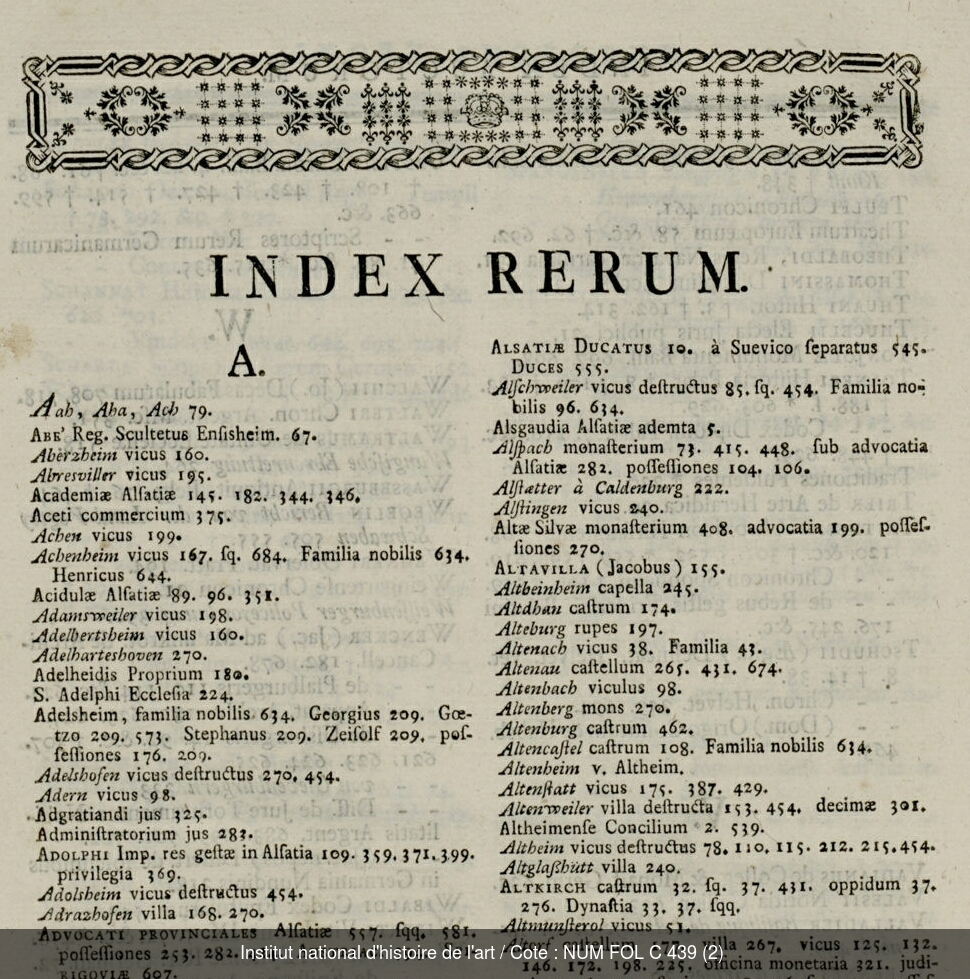
\includegraphics[width=6cm]{images/index_rerum_alsatia.jpg}
		\caption{Index rerum}
	\end{minipage} 
	\medskip
	Extraits des deux index de l'œuvre de \nP{Jean-Daniel}{Schoepflin} [Source: \url{http://bibliotheque-numerique.inha.fr/idurl/1/12532}, p.804 et 813]
\end{figure}

\chapter{\label{annexe_types_interop}Les différents types d'interopérabilité}
\titreEntete{Annexe \thechapter}

\begin{figure}[!h]
	\centering
	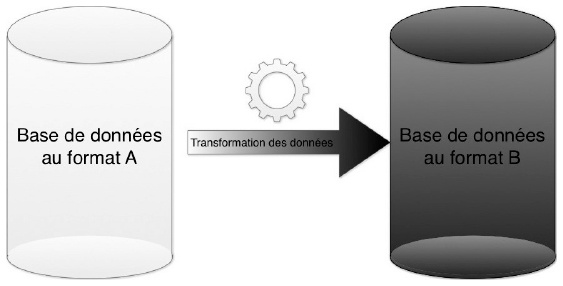
\includegraphics[width=12cm]{images/interop_conversion_copie.jpeg}
	\medskip
	\caption[L'interopérabilité par conversion et copie]{L'interopérabilité par conversion et copie [Source: \cite{bermes_2_2013}]}
\end{figure}

\begin{figure}[!h]
	\centering
	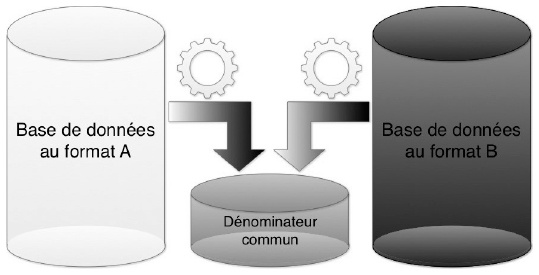
\includegraphics[width=12cm]{images/interop_denom_commun.jpeg}
	\medskip
	\caption[L'interopérabilité par le plus petit dénominateur commun]{L'interopérabilité par le plus petit dénominateur commun [Source: \cite{bermes_2_2013}]}
\end{figure}
	
	\backmatter
	
	
%bibliographie ici dans les normes de l'école
%\printbibliography[title= Bibliographie sélective, prenote=intro]%postnote est aussi possible
%\printbibliography[heading=subbibliography, keyword={semantique}, title={Sémantique}]%biblio sélective pour un mot clé donné

\printindex[referentiels]
\printindex[ina]

	\listoffigures

	\tableofcontents
	
\end{document}